\documentclass{article}
\usepackage[english]{babel}
\usepackage{graphicx,textcomp,hyperref}

%%%%%%%%%% Start TeXmacs macros
\newcommand{\assign}{:=}
\newcommand{\tmem}[1]{{\em #1\/}}
\newcommand{\tmtextbf}[1]{{\bfseries{#1}}}
\newcommand{\tmtextit}[1]{{\itshape{#1}}}
\newcommand{\tmtexttt}[1]{{\ttfamily{#1}}}
%%%%%%%%%% End TeXmacs macros

\begin{document}

\title{Branching ratio approximation for the self-exciting Hawkes process}

\author{
  Stephen J. Hardiman
  \and
  Jean-Philippe Bouchaud
}

\date{April 9, 2015}

\maketitle

\begin{abstract}
  We introduce a model-independent approximation for the branching ratio of
  Hawkes self-exciting point processes. Our estimator requires knowing only
  the mean and variance of the event count in a sufficiently large time
  window, statistics that are readily obtained from empirical data. The method
  we propose greatly simplifies the estimation of the Hawkes branching ratio,
  recently proposed as a proxy for market endogeneity and formerly estimated
  using numerical likelihood maximisation. We employ our new method to support
  recent theoretical and experimental results indicating that the best fitting
  Hawkes model to describe S\&P futures price changes is in fact critical (now
  and in the recent past) in light of the long memory of financial market
  activity.
\end{abstract}

\section{The self-exciting Hawkes Process}

The Hawkes model {\cite{hawkes,hawkes2}} is a simple and powerful framework
for simulating or modelling the arrival of events which cluster in time (e.g.
earthquake shocks and aftershocks, neural spike trains and transactions on
financial markets). In one dimension, the model is a counting process $N (t)$
with an intensity $\lambda (t)$ (the expected number of events per unit time)
given by a constant term ${\textmu}$ and a `self-exciting' term which is a
function of the event history.
\begin{equation}
  \lambda (t) ={\textmu}+ \int_{- \infty}^t \phi (t - s) \mathrm{d} N (s)
  \label{eq:hawkes}
\end{equation}
This self-exciting term gives rise to event clustering through an endogenous
feedback: past events contribute to the rate of future events. $\phi (\tau)
\geq 0$ is the ``influence kernel'' which decides the weight to attribute to
events which occurred at a lag $\tau$ in the past. The base intensity
${\textmu}$ and the kernel shape $\phi (t)$ are parameters to be varied. A
popular choice for the kernel is the exponential function $\phi (\tau) =
\alpha e^{- \beta \tau}$ {\cite{filimonov,ozaki}} but in general the kernel to
be used should depend on the application or the dynamics of the data to be
modelled. Note that for $\phi (t) = 0$ the model reduces to a Poisson process
with constant intensity ${\textmu}$.

By taking the expectation of both sides of Eq. (\ref{eq:hawkes}) and assuming
stationarity (i.e. a finite average event rate $E [\lambda (t)] = \Lambda$),
we can express the average event rate of the process as $\Lambda ={\textmu}/
(1 - n) \geq {\textmu}$ where $n = \int \phi (\tau) \mathrm{d } \tau$. One can
create a direct mapping between the Hawkes process and the well known
branching process {\cite{harris}} in which exogenous ``mother'' events occur
with an intensity ${\textmu}$ and may give rise to $x$ additional endogenous
``daughter'' events, where $x$ is drawn from a Poisson distribution with mean
$n$. These in turn may themselves give birth to more ``daughter'' events, etc.

The value $n$, which corresponds with the integral of the Hawkes kernel is the
branching ratio, determines the behaviour of the model. If $n > 1$, meaning
that each event typically triggers at least one extra event, then the process
is non-stationary and may explode in finite time
{\cite{commodityreflexivity}}. However, for $n < 1$, the process is stationary
and has proven useful in modelling the clustered arrival of events in a wide
variety of applications including neurobiology {\cite{neurobiology}}, social
dynamics {\cite{social,crime}} and geophysics
{\cite{earthquakes1,earthquakes2}}. The Hawkes model has also seen many recent
applications to finance {\cite{bauwens,hawkesvolatility,bormetti}}, especially
as a means of modelling the very high-frequency events affecting the
limit-order book of financial exchanges
{\cite{bacry,hawkesmicrostructure,bacrypricetrades,toke,dafonseca}}.

One novel application of the Hawkes framework to finance is as a means of
measuring market endogeneity or `reflexivity' in financial markets
{\cite{filimonov,commodityreflexivity}}. In {\cite{filimonov}}, the authors
consider mid-price changes in the E-mini S\&P Futures contract between 1998
and 2010 and observe that the branching ratio $n$ of the best-fitting
exponential kernel model has been increasing steadily over this period, from
$n \approx 0.25$ in 1998 to $n \approx 0.65$ in 2010 (see our Fig. 6 below).
They argue that this observation implies that the market has become more
reflexive in recent years with the rise of high frequency and algorithmic
trading and is therefore more prone to market instability and so-called
``flash crashes''.

In {\cite{criticalreflexivity}}, however, we have argued that due to the
presence of long-range dependence in the event rate of mid-price changes
(detectable in both 1998 and 2011) as one extends the window of observation,
the best fitting stationary Hawkes model must in fact be critical, i.e. have a
branching ratio $n = 1$. This is backed up by theoretical arguments and
empirical measurements on market data.

Let us however insist that this conclusion only holds if one believes that
Hawkes processes provide an exact representation of the reality of markets. It
is very plausible that the dynamics of markets is more complicated (and
involves, for example, non-linearities absent from the Hawkes process defined
by Eq. (\ref{eq:hawkes})), but that the best way to represent this dynamics
within the framework of Hawkes processes is to choose $n = 1$ with a
long-ranged influence kernel.

In this article we introduce a simple approximation for the branching ratio of
the Hawkes process which allows us to faithfully reproduce the results of
{\cite{filimonov}} which proposes the statistic as a measure of market
instability and as a crash prediction metric. The interest of our
approximation lies in its great simplicity: one need only estimate the mean
and variance of the event count in a sufficiently large time window. The
approximation also avoids a number of pitfalls {\cite{apparentcriticality}}
inherent to the significantly more complex approach {\cite{ozaki}} employed in
{\cite{filimonov}}.

The estimator accepts one parameter, a time window size, $W$, during which we
measure the mean and variance of the event count. We note that when we employ
our estimator to mid-price changes in the S\&P electronic futures market with
a fixed window size $W$ then the branching ratio estimate obtained increases
over time as reported in {\cite{filimonov}}. If, however, we allow the window
size to scale appropriately (halving in size every 18 months) to adapt to the
decreasing latency of interactions on the market we recover a constant
branching ratio estimate as proposed in {\cite{criticalreflexivity}}. This
result reiterates the need for a scale-invariant, or at least scale-sensitive
means of measuring the `reflexivity' of financial market events.

\section{Maximum likelihood estimation}

Given observed events (e.g. mid-price changes) at times $t_1, t_2, \ldots,
t_n$ in an interval $[0, T]$ one can fit the Hawkes model by maximising the
log-likelihood {\cite{rubin,ozaki}} over the set of parameters $\theta$.
\begin{equation}
  \log L (t_1, \ldots, t_n | \theta) = - \int_0^T \lambda (t| \theta)
  \mathrm{d} t + \int_0^T \log \lambda (t| \theta) \mathrm{d} N (t)
  \label{eq:loglikelihood}
\end{equation}
In the case of the exponential kernel $\theta = \{{\textmu}, \alpha, \beta\}$.
In practice, the model parameters $\{ \hat{{\textmu}}, \hat{\alpha},
\hat{\beta} \}$ which maximise this log-likelihood are obtained with numerical
techniques due to the lack of a closed form solution \footnote{Note that the
method above is not the only method proposed to fit the parameters of the
Hawkes process for financial applications, indeed a recent publication
{\cite{dafonseca}} proposes a fast albeit still parametric method for fitting
the multivariate exponential Hawkes process.}. The branching ratio estimate is
then $\hat{n} = \hat{\alpha} / \hat{\beta}$.

However, there are a number of pitfalls to using this procedure as a means of
estimating the Hawkes branching ratio $n = \int \phi (\tau) \mathrm{d} \tau$
{\cite{apparentcriticality}}. Arguably the most important of which is that any
estimate of $n$ made in this manner will be heavily dependent on the choice of
kernel model (e.g. exponential, power-law, etc.) It may be that the chosen
model cannot satisfactorily describe the observed events, hence the meaning of
the branching ratio extracted from the maximum likelihood method is
questionable.

Care must also be taken when employing this method in the presence of
imperfect event data as illustrated in {\cite{apparentcriticality}}. In one of
their figures, the authors present a (negative) log-likelihood surface which
features two minima (one local, and one global). The global log-likelihood
minimum does in fact little more than describe packet clustering inside the
millisecond which arises from the manner in which events arriving at the
exchange at different times are bundled and recorded with the same timestamp.
Subsequent randomisation of the timestamps inside a short time interval (in
this case, one millisecond) creates a spurious high frequency correlation,
that makes the global minimum irrelevant. The local log-likelihood minimum,
which is in fact a better fit to the `true' lower frequency dynamics, does a
poor job at explaining the spurious high frequency clustering and is punished
with a lower log-likelihood. Indeed, when the authors of
{\cite{apparentcriticality}} choose to fit this local minimum they corroborate
results presented in {\cite{criticalreflexivity}}.

We believe it is therefore essential to have additional checks (such as
non-parametric methods {\cite{bacry}}) at one's disposal to support results
obtained from likelihood maximisation. To address the pitfalls in branching
ratio estimation that arise from the model choice we propose a simple
model-independent tool for branching ratio approximation, in the next section,
which accurately reproduces previous results of {\cite{filimonov}} and also
indicates the criticality of the relevant Hawkes process which describes the
market.

\section{A mean-variance estimator for the branching ratio $n$}

We begin with a general expression relating the Fourier transform of the
kernel function to the Fourier transform of the auto-covariance $\nu (\tau) =
E [\frac{\mathrm{d} N (t) \mathrm{d} N (t + \tau)}{\mathrm{d} t^2}] -
\Lambda^2$ of the event rate. (see {\cite{hawkes,bacry}} for a derivation).
\begin{equation}
  \hat{\nu} (\omega) = \frac{\Lambda}{| 1 - \hat{\phi} (\omega) |^2}
\end{equation}
Setting $\omega = 0$ we obtain a relation between the branching ratio, the
average event rate and the integral of the auto-covariance (in the stationary
case $n \leq 1$)
\begin{equation}
  \label{basic} \int_{- \infty}^{\infty} \nu (t) \mathrm{d} t =
  \frac{\Lambda}{\left| 1 - \int_0^{\infty} \phi (t) \mathrm{d} t \right|^2}
  \equiv \frac{\Lambda}{(1 - n)^2}
\end{equation}
Therefore, to deduce the branching ratio of the stationary Hawkes process, we
need only find the value of $\Lambda$ and $\int_{- \infty}^{\infty} \nu (t)
\mathrm{d} t$. Estimating $\Lambda$ is trivial, it is given by the empirical
average number of events per unit time. To estimate $\int_{- \infty}^{\infty}
\nu (t) \mathrm{d} t$, we consider the variance of the total event count $N_W$
in a window of length $W$. Theoretically, this is given by:
\begin{eqnarray}
  \sigma^2_W & = & \mathrm{E} \left[ \int_{t = 0}^W \frac{\mathrm{d} N
  (t)}{\mathrm{d} t} \mathrm{d} t \int_{t' = 0}^W \frac{\mathrm{d} N
  (t')}{\mathrm{d} t'} \mathrm{d} t' \right] - (\Lambda W)^2 \nonumber\\
  & = & \int_{t = 0}^W \int_{t' = 0}^W \nu (t - t') \mathrm{d} t
  \hspace{0.17em} \mathrm{d} t' \nonumber\\
  & = & \int_{t = 0}^W \int_{\tau = - t}^{W - t} \nu (\tau) \mathrm{d} t
  \hspace{0.17em} \mathrm{d} \tau \nonumber\\
  & = & \int_{\tau = - W}^W \nu (\tau)  (W - | \tau |) \mathrm{d} \tau
  \nonumber\\
  & \leq & W \int_{- \infty}^{\infty} \nu (\tau) d \tau  \label{eq:bounded}
\end{eqnarray}
We then note that provided:
\begin{enumerate}
  \item $\nu (t) \to 0$ for $|t| > R$
  
  \item $W \gg R$ such that $(W - |t|) / W \approx 1$ for all $|t| < R$
\end{enumerate}
then
\begin{equation}
  \sigma^2_W \approx W \int_{\tau = - \infty}^{\infty} \nu (\tau) \mathrm{d}
  \tau \label{eq:covariance}
\end{equation}
and we find, using Eq. (\ref{basic}):
\begin{eqnarray}
  n \approx & 1 - \sqrt{\frac{{\textmu}_W}{\sigma^2_W}} \assign \tilde{n} 
  \label{eq:simple}
\end{eqnarray}
where ${\textmu}_W = \Lambda W$ is the average number of events falling in a
window of size $W$. The above expression has a very intuitive interpretation.
When the variance is equal to the event rate, the process is obeying Poisson
statistics and $n = 0$. Any increase in the variance above the event rate
indicates some positive correlations and, within a Hawkes framework, a
positive branching ratio.

Note from Eq. (\ref{eq:bounded}) that $\sigma^2_W / W$ is a biased estimator
for $\int_{- \infty}^{\infty} \nu (\tau)$ and for a general $W$ will fall
short of its theoretical value. This means that Eq. (\ref{eq:simple}) will
generally under-estimate the branching ratio and only become exact in the
limit $W \to \infty$.

In practice, to estimate the branching ratio of an empirical sample of total
length $T = mW$ we substitute the mean and variance term in Eq.
(\ref{eq:simple}) by their sample estimates:
\begin{eqnarray}
  \tilde{{\textmu}}_W = W \frac{N_T}{T} \equiv \frac{1}{m}  \sum_{i = 1}^m N_W
  (i) \\
  \tilde{\sigma}^2_W = \frac{1}{m - 1}  \sum_{i = 1}^m (N_W (i) -
  \tilde{{\textmu}}_W)^2  \label{eq:variance}
\end{eqnarray}
An estimate obtained in this fashion is asymptotically convergent for large $T
\gg W$, i.e. $m \gg 1$. For a fixed window size $W$ we can always ensure that
our estimate of the variance of $N_W$ is within a desired maximum error with a
desired minimum probability by increasing $T$ and therefore the number of
observations $m$ of $N_W$. Furthermore, we can make Eq. (\ref{eq:covariance})
exact by allowing $W$ to be arbitrarily large.

Note, however, that for any finite $m$, the average of $\tilde{n}$ over all
possible realisations of the process is in fact $- \infty$! This is because a
value $\tilde{\sigma}^2_W = 0$ is always possible with a non zero probability.
For this reason we choose to present the median of our estimates.

\section{Numerical simulations \& Implementation notes}

In Fig. \ref{fig:varying}, we test the estimation procedure described in the
previous section on a number of simulated exponential Hawkes processes with a
variety of branching ratios. To do this we fix $\beta = 1.0$ but vary $\alpha
= n$ in the range $0 \leq \alpha \leq 0.95$. We choose a base intensity
${\textmu}= 1 - n$ such that each process has the same average event rate
$\Lambda = 1$. We simulate the process for a time $T = 10^5$ using simulation
Algorithm 1 described in {\cite{moller2005perfect}}. This procedure is prone
to edge effects so we disregard the initial period of size $10^4$ to ensure
the process is close to stationarity in the period studied.

We estimate the branching ratio with a window size $W = 20$ significantly
larger than the time-scale of correlation of our process $\beta^{- 1} = 1$.
However, the window size chosen is also sufficiently small that we have a
significant number of independent observations $m = (0.9 \times 10^5) / 20$
with which to make a reliable estimate of the variance of $N_W$. We see very
good agreement between our branching ratio estimates and the input branching
ratio of the simulation, see Fig. \ref{fig:varying}.

Note however, that our approximation systematically underestimates the
branching ratio since our finite window size does not completely cover the
region of support of the autocorrelation function. This is particularly
visible in Fig. \ref{fig:varying} for large $n$. We now investigate the effect
of window size on the estimate obtained.

\begin{figure}[h]
  \resizebox{1tex-column-width}{!}{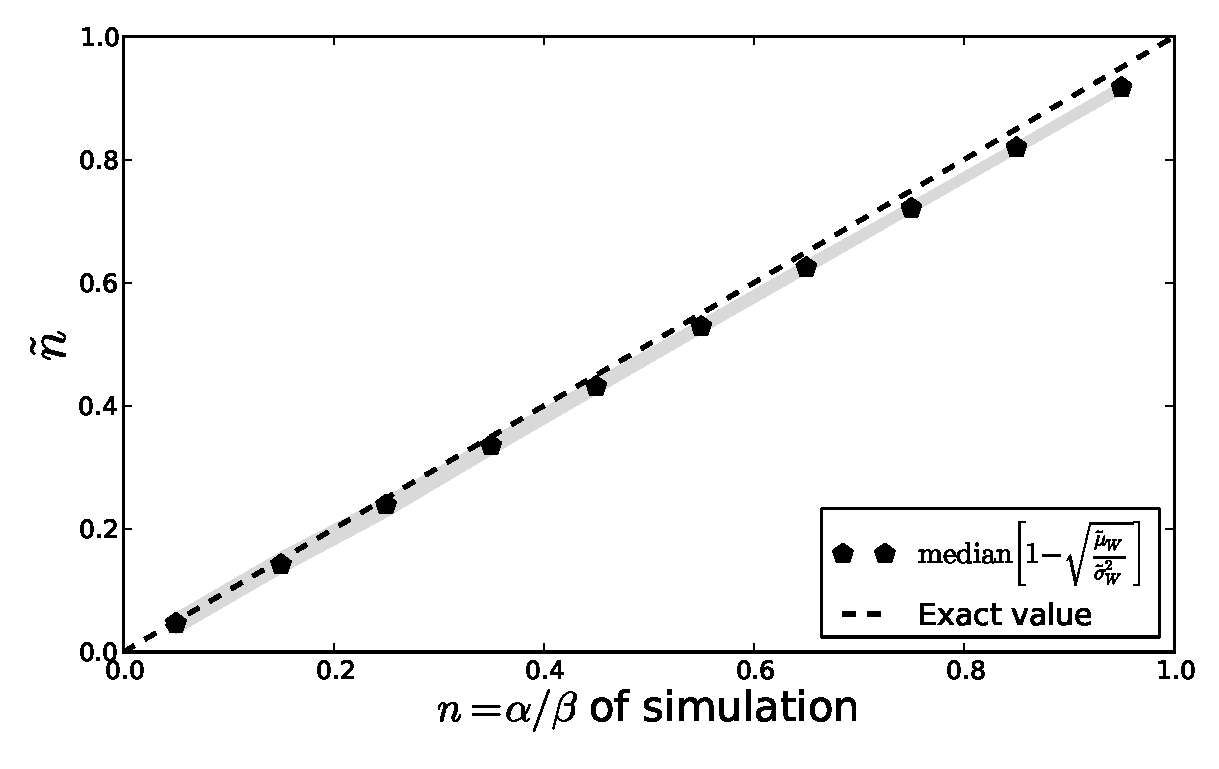
\includegraphics{varying_n_20.pdf}}
  \caption{\label{fig:varying} Applying the mean-variance branching ratio
  approximation method to a simulated Hawkes process with exponential kernel
  form and scale parameter $\beta = 1.0$. $\alpha$ is varied to decide the
  branching ratio, and ${\textmu}$ is varied to keep the average event rate
  fixed at $\Lambda = 1.0$. The process is simulated for $T = 100000 s$ and
  the branching ratio estimate is made using Equation \ref{eq:simple} with a
  window size $W = 20$. The mean and [5\%,95\%] confidence bands are
  calculated over an ensemble of 100 process for each parameter set.}
\end{figure}

\subsection{Choice of window size W}

For Eq. (\ref{eq:covariance}) to be accurate, we must choose a large $W$.
However for a finite sample size, large $W$ implies small $m = (T / W)$ and
therefore less statistical power with which to estimate the variance of the
event count $N_W$. This compromise is illustrated in Fig. \ref{fig:varying}
for which we simulate an ensemble of exponential Hawkes processes with
parameters $\alpha = 0.75$, $\beta = 1.0$ and ${\textmu}= 0.25$. We note that
for increasing window size $W$, the confidence bands of our estimate converge
on the expected value of $n = 0.75$.

However when we make the window size too large, we suffer significant error
coming from the estimation of the variance. For the practical implementation
of this procedure to empirical data we recommend a choice of window size
sufficiently large to capture the bulk of autocorrelation present in the event
rate, but sufficiently small that one can expect to obtain reliable estimates
of the variance of the event count in that window.

One can approximate upper and lower confidence intervals on the branching
ratio estimate from a single realisation of a time series by bootstrap
re-sampling. Indeed the simple variance estimator of Eq. (\ref{eq:variance})
is not optimal and can be improved with the use of over-lapping windows or,
for example, a Monte Carlo sampling scheme which selects random windows with
replacement.

\begin{figure}[h]
  \resizebox{1tex-column-width}{!}{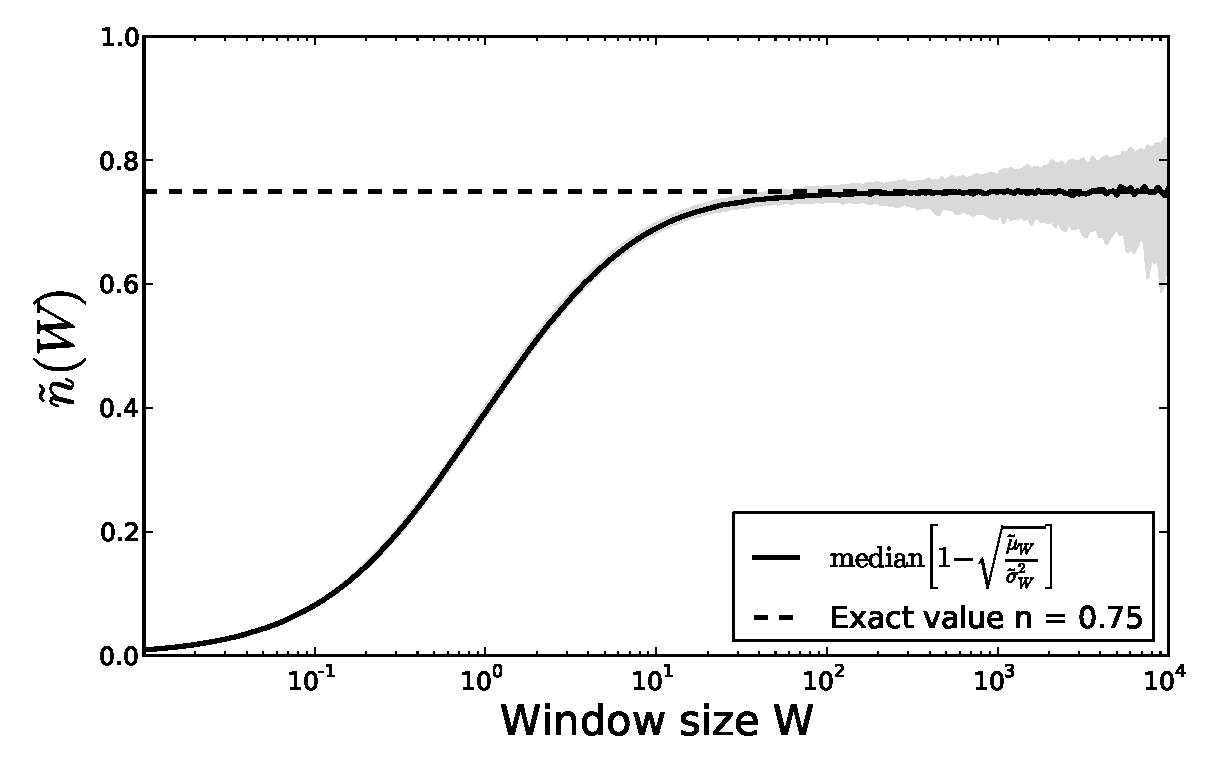
\includegraphics{varying_W_simulation.pdf}}
  \caption{\label{fig:varying} Applying the mean-variance branching ratio
  approximation method to simulated data. Shaded area represents the
  [5\%,95\%] confidence interval. We note that the branching ratio estimate
  converges on the expected value of $0.75$ as the window size increases. For
  very large W, we lack a sufficient number of event count observations to
  estimate the variance of $N_W$ with precision and the confidence interval
  grows considerably.}
\end{figure}

\subsection{Power-law kernel}

Finally we test the estimation procedure on a (near) critical power-law Hawkes
process, a type suggested in some recent publications as a good fit to
financial event data {\cite{bacry,criticalreflexivity}}. Specifically, we
consider a kernel with an Omori law form:
\[ \phi (\tau) = \frac{n \epsilon \tau_0^{\epsilon}}{(\tau_0 + \tau)^{(1 +
   \epsilon)}} \]
In the critical case of $n = 1$ with $0 < \epsilon < 0.5$ this process will
exhibit long-range dependence, with an autocorrelation function $\nu (\tau)$
decaying asymptotically as a power law: $\nu (\tau) \sim \tau^{- (1 - 2
\epsilon)}$ {\cite{bremaud,criticalreflexivity}}. The integral of the
autocorrelation function is therefore divergent for large $\tau$'s and the
variance of the event count in a window of size $W$ grows with as $\sigma^2_W
\sim W^{1 + 2 \epsilon}$. The $\sqrt{\frac{{\textmu}_W}{\sigma^2_W}}$ term in
Eq. \ref{eq:simple} will in this case not converge to a finite constant for
large $W$ but rather shrink to zero, leading to $1 - \tilde{n} \sim W^{-
\epsilon}$.

We have simulated such a process with exponent $\epsilon = 0.35$ and cut-off
parameter $\tau_0 = 1.0$. To allow our simulation to attain a stationary state
with an average event rate $\Lambda \approx 1$, we make our process very near
critical by choosing $n = 0.99$ and ${\textmu}= 0.01$. We simulate for a very
long period $T = 1 \times 10^9$ and discard the first $0.9 \times 10^9$ to
ensure the process is close to stationarity ($\Lambda > 0.99$ at $0.9 \times
10^9$). In Fig. \ref{fig:power} we present the results of branching ratio
estimation using Eq. (\ref{eq:simple}) with a variety of window sizes $W$.

We note that the branching ratio estimate we obtain is very much dependent on
the choice of window size used. To capture all the correlation present in the
process and obtain estimates close to the the true input value $n = 0.99$ we
must probe the correlation on very large scales, by choosing a very large
value for $W$. The branching ratio obtained indeed varies with window size
according to the law $W^{- \epsilon}$, in a similar way to the integral of the
kernel $\phi (\tau)$, see Fig. \ref{fig:power}.

\begin{figure}[h]
  \resizebox{1tex-column-width}{!}{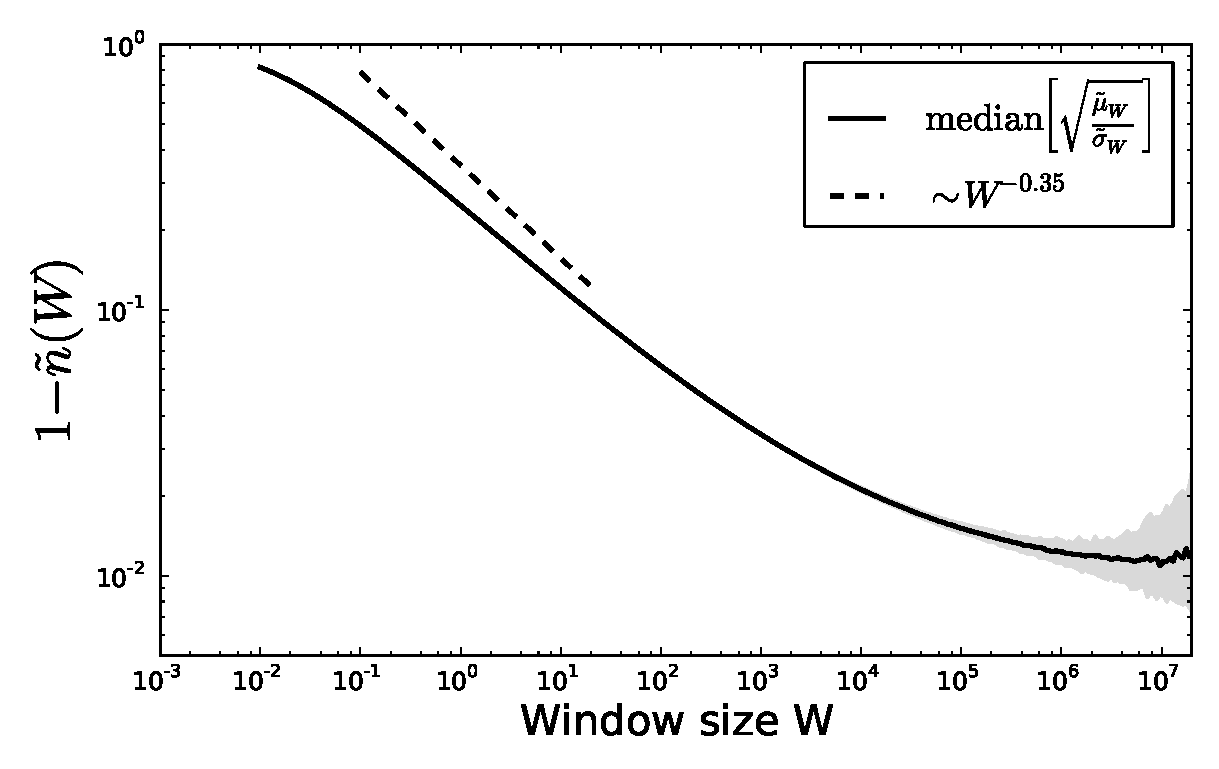
\includegraphics{power_law.pdf}}
  \caption{\label{fig:power} $1 - \tilde{n}$ for simulated near-critical ($n
  = 0.99, \epsilon = 0.35$) power-law Hawkes processes. The value for $1 -
  \tilde{n}$ that we obtain approximately scales as $\sim W^{- 0.35}$ for
  large $W$. Note that the simulated process is only `near-critical' (with a
  branching ratio $n = 1 - 1 \times 10^{- 2}$) so for very large $W$ the curve
  levels off and converges to $1 \times 10^{- 2}$.}
\end{figure}

\section{Empirical applications}

\subsection{Flash-crash revisited}

To demonstrate the effectiveness of this simple estimator we have repeated the
flash-crash day branching ratio analysis of Filimonov \& Sornette
{\cite{filimonov}}. We consider non-overlapping periods of 10 minutes in the
hours of trading before and just after the flash-crash. For each 10-minute
period, we calculate the sample mean and variance of the number of mid-price
changes in the 60 windows of length $W = 10 s$ contained. The resulting values
are plugged into Eq. (\ref{eq:simple}) to obtain an approximation of the
branching ratio for each period. The results are presented in Fig.
\ref{fig:flashcrash}.

\begin{figure}[h]
  \resizebox{1tex-column-width}{!}{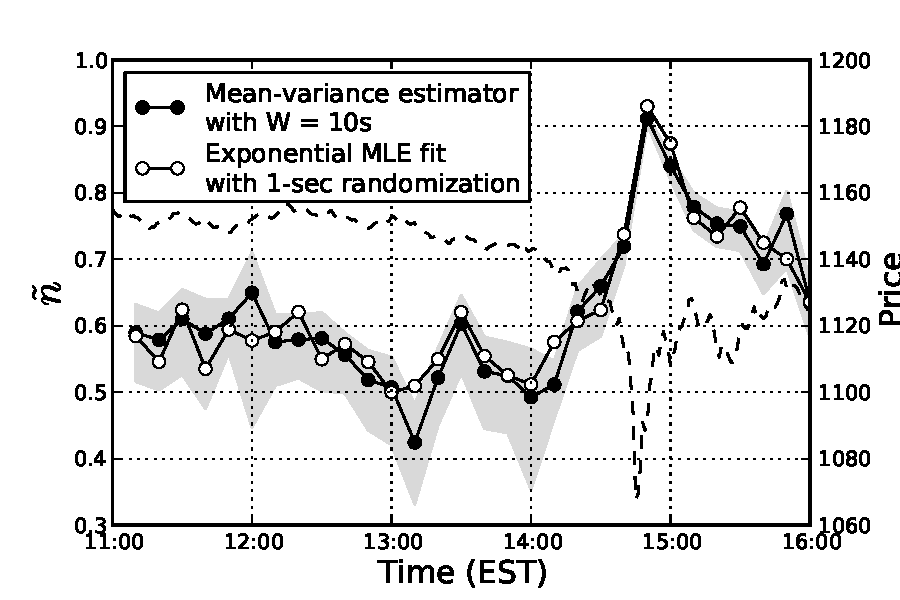
\includegraphics{flashcrash.pdf}}
  \caption{\label{fig:flashcrash} Reproduction of the flash-crash branching
  ratio analysis of Filimonov \& Sornette using the mean-variance estimator.
  Our results compare well with those obtained by maximising the likelihood of
  the exponential model (with 1-second randomisation). The dashed line is the
  E-mini S\&P price. The points are placed at the end of the 10-minute period
  for which the branching ratio estimate is made. The shaded region is a
  [10\%,90\%] confidence interval generated by bootstrap re-sampling.}
\end{figure}

Note that this simple estimator is biased, and for a general $W$, will
typically underestimate the value of $\int_{- \infty}^{\infty} \nu (t)
\mathrm{d} t$ and therefore the branching ratio. Since we consider a window
size $W = 10 s$ we have systematically underestimated $n$ in Figure
\ref{fig:flashcrash} as measurements of $\nu (t)$ on this data have support
outside the interval $[- 10 s, 10 s]$ ---  there is still significant
autocorrelation in the event rate at scales longer than $10 s$.

However, we have identified that a window size $W$ of the order of
approximately 10 to 30 seconds produces estimates of the branching ratio on
our data in line with those obtained by ML fitting to the exponential model
after intra-second randomisation (the method applied in {\cite{filimonov}}.)
Note that we do not fix $\beta$ in our ML fit but let it settle naturally at
the value which maximises the log-likelihood. We observe that this value
$\hat{\beta}$ is very much dependent on the period of
randomisation\footnote{To address the limited precision of the event data in
{\cite{filimonov}}, the authors randomise timestamps uniformly inside the
second that they are reported.} of the timestamps. When we randomise
timestamps inside each millisecond we obtain $\hat{\beta}^{- 1} \approx 10^{-
2}$ for periods in 2010 but randomisation at larger intervals (e.g. the
intra-second randomisation of Filimonov \& Sornette) prevents $\hat{\beta}^{-
1}$ from exceeding values of the order of magnitude of the scale of
randomisation.

Note that since our results with $W = 10 s$ correspond well with those
obtained using the methods of Filimonov \& Sornette {\cite{filimonov}}, their
procedure must {\tmem{also}} underestimate the branching ratio. To converge on
the true $n$ in expectation, we must take Eq. (\ref{eq:simple}) in the limit
of $W \to \infty$. We do just this in Fig. \ref{fig:n} for mid-price changes
of the E-mini S\&P Futures contract in 2010. One notes that as the window size
increases, the branching ratio converges to $n = 1$ in a non-trivial way. As
reported in {\cite{criticalreflexivity}} for the structure of the kernel at
short and long time-scales, two regimes are detectable with a transition
around five minutes. The branching ratio asymptotically tends towards $n =
1.0$ with a scaling exponent $\epsilon = - 0.37$ compatible with the value of
$0.45$ estimated in {\cite{criticalreflexivity}} for a 14-year period. Note
that in taking the limit $W \to \infty$ we consider variation in the event
rate at significant time-scales to be explained by the stationary Hawkes
model.

\begin{figure}[h]
  \resizebox{1tex-column-width}{!}{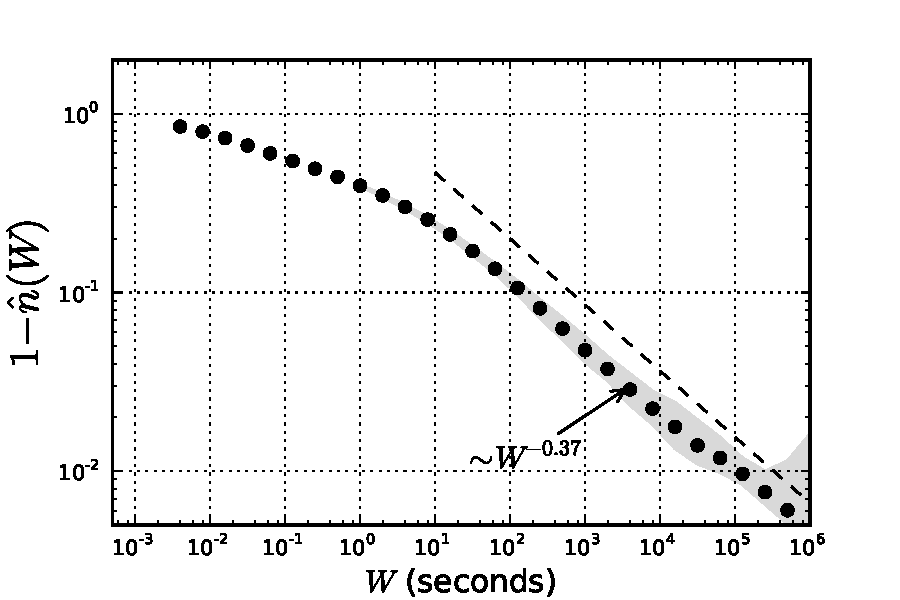
\includegraphics{n_2010.pdf}}
  \caption{\label{fig:n} $1 - \tilde{n}$, the estimate of the branching ratio
  as a function of window size for E-mini S\&P mid-price changes in 2010. The
  mean and variance of $N_W$ are estimated on the full year. The change of
  power-law behaviour occurs around $100$ seconds. Note that we have
  `stitched' together all 5-minute bins of regular trading hours (09:30 to
  16:00 EST) that contain at least one event (this solves a problem arising
  from missing data at half-days). We have then de-trended the intra-day
  seasonality by dividing each 5-minute event count by a normalised average
  event rate for each 5-minutes of the trading day calculated on the full
  year.}
\end{figure}

\subsection{Reflexivity : 1998 - 2013}

Using the mean-variance estimator, we can also easily reproduce the result of
{\cite{filimonov}} that claims to demonstrate that reflexivity has been
increasing in the S\&P futures market since 1998. To do this we set our only
parameter $W = 30 s$ and estimate the branching ratio in periods of
15-minutes. In Fig. \ref{fig:19982013} we present the 2-month medians of these
estimates beside the median of the branching ratio estimate obtained using the
exponential maximum likelihood approach after intra-second randomisation.

\begin{figure}[h]
  \resizebox{1tex-column-width}{!}{\includegraphics{1998_to_2013.pdf}}
  \caption{\label{fig:19982013} Estimates of the branching ratio for
  15-minute windows using the method of Filimonov \& Sornette
  {\cite{filimonov}} and estimates using the mean-variance estimator with a
  window size of $W = 30 s$. Note that our MLE results differ somewhat from
  the plot presented in {\cite{filimonov}}. We attribute this to differences
  in the data source or identification of mid-price changes.}
\end{figure}

Since we expect the minimum time-scale of correlation in the data to have
decreased over the past decades (due to decreasing latency with advancing
technology) we now re-perform the experiment but with a window size $W_t$ that
follows Moore's law in such a way to keep the average number of events in
$W_t$ roughly constant. More precisely the window size $W_t$ halves every 18
months; this describes well the increase in the high frequency activity of
markets, see {\cite{criticalreflexivity}}. The results of this experiment are
presented in Fig. \ref{fig:varying} and confirm that the kernel integral is
approximately invariant over time provided that the measurement window $W_t$
is appropriately rescaled to account for the changing speed of interactions in
the market. We find this quite remarkable, as this suggests that the amount of
self-reflexivity in financial markets is \tmtextit{scale invariant}, and has
not significantly increased due to high-frequency trading.

\begin{figure}[h]
  \resizebox{1tex-column-width}{!}{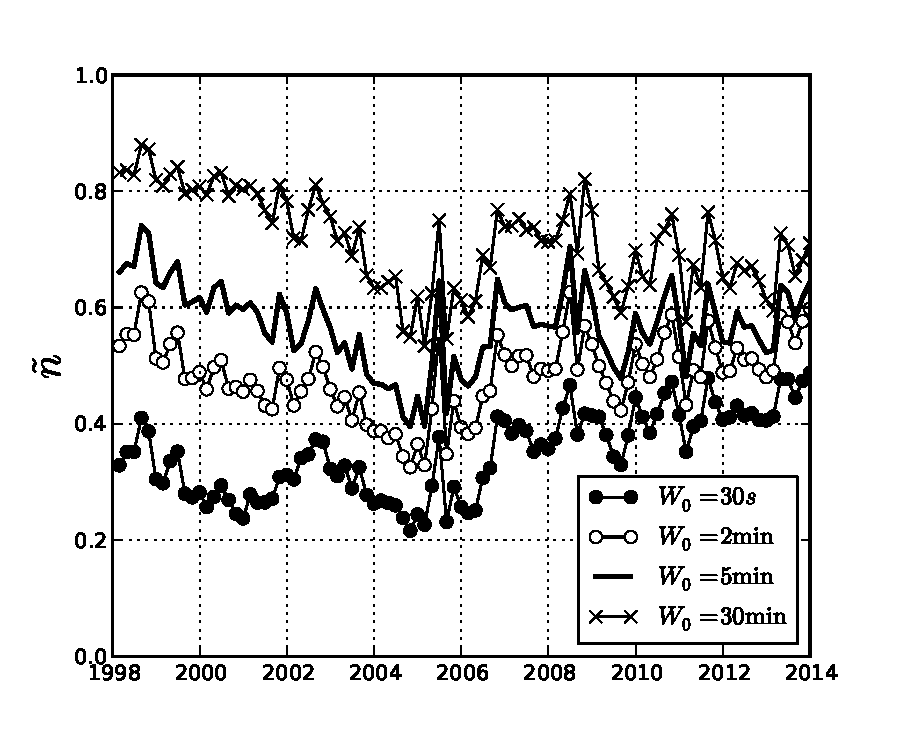
\includegraphics{varying_W.pdf}}
  \caption{\label{fig:varying} Estimates of the branching ratio on 2-month
  periods using the mean-variance estimator with a window size that follows
  Moore's law: $W_t = W_0 e^{- c (t - t_0)}$ with $c = - \log (1 / 2) / (18
  \hspace{0.17em} \mathrm{months})$ and $t_0 = 1998$. We again stitch together
  periods of regular trading hours and de-trend the event count by the
  intra-day U-shape for each year. When $W$ is appropriately rescaled, the
  branching ratio estimate is approximately constant through time, for all
  values of $W_0$, and tends to $n = 1.0$ for large $W_0$.}
\end{figure}

\section{Summary}

We have introduced a simple estimator for the branching ratio of Hawkes
self-exciting point-process. The method is straight-forward to apply to
empirical event data since it requires only a rudimentary calculation on the
mean and variance of the event rate. The estimator does not suffer from the
bias inherent to the contentious question of the choice of kernel in the
likelihood maximisation approach, and furthermore it avoids the need for
complicated numerical minimisation techniques.

Despite its simplicity, our estimator can accurately reproduce results
obtained for the branching ratio using this prior method. The estimator
presented is indeed a biased estimator, but it can be made asymptotically
unbiased in the limit of large $W$ and $T$, for which we observe that the
branching ratio for empirical mid-price changes of the E-mini S\&P futures
contract approaches unity in line with previous theoretical and empirical
results {\cite{criticalreflexivity}}.

Furthermore we demonstrate that if the window size is allowed to scale with
Moore's law and adapt to the changing speed of interaction in the market over
the past fifteen years, then the branching ratio approximation recovered is
constant supporting prior observations of the invariance of the Hawkes kernel
and branching ratio over time in {\cite{criticalreflexivity}}.

Finally, let us reiterate the caveat made above: the Hawkes analysis of the
activity in financial markets leads to the conclusion that the process must be
critical. However, it might well be that the dynamics of markets is more
complicated and requires non-linearities absent from the Hawkes process
defined by Eq. (\ref{eq:hawkes})). More work on this issue would be highly
interesting, and is in progress in our group.

\section*{Acknowledgements}

We thank V. Filimonov for many productive discussions about this topic. We are
also indebted to N. Bercot, J. Kockelkoren, M. Potters, I. Mastromatteo, P.
Blanc and J. Donier for interesting and useful comments.

\begin{thebibliography}{10}
  \bibitem[1]{hawkes}A.~G. Hawkes, ``Spectra of some mutually exciting point
  processes,'' \tmtextit{Biometrika} \tmtextbf{58} (1970) 83.
  
  \bibitem[2]{hawkes2}A.~G. Hawkes, ``Point spectra of some mutually exciting
  point processes,'' \tmtextit{Journal of the Royal Statistical Society,
  Series B} \tmtextbf{33} no.~3, (1971) 438--443.
  
  \bibitem[3]{filimonov}V.~Filimonov and D.~Sornette, ``Quantifying
  reflexivity in financial markets: Toward a prediction of flash crashes,''
  \tmtextit{Physical Review E} \tmtextbf{85} (2012) 056108.
  
  \bibitem[4]{ozaki}T.~Ozaki, ``Maximum likelihood estimation of Hawkes
  self-exciting point process,'' \tmtextit{Annals of the Institute of
  Statistical Mathematics} \tmtextbf{31} (1979) 145--155. Part B.
  
  \bibitem[5]{harris}T.~E. Harris, \tmtextit{The Theory of Branching
  Processes}. {\newblock}Dover Publications, 2002.
  
  \bibitem[6]{commodityreflexivity}V.~Filimonov, D.~Bicchetti, N.~Maystre, and
  D.~Sornette, ``Quantification of the high level of endogeneity and of
  structural regime shifts in commodity markets.,'' \tmtextit{Journal of
  International Money and Finance} \tmtextbf{42} (April, 2013) 174--192.
  
  \bibitem[7]{neurobiology}V.~Pernice, B.~Staude, S.~Cardanobile, and
  S.~Rotter, ``How structure determines correlations in neuronal networks,''
  \tmtextit{PLOS Computational Biology} \tmtextbf{7} (2011) e1002059.
  
  \bibitem[8]{social}R.~Crane and D.~Sornette, ``Robust dynamic classes
  revealed by measuring the response function of a social system,''
  \tmtextit{Journal of the American Statistical Association} \tmtextbf{105}
  no.~41, (September, 2008) 15649--15653.
  
  \bibitem[9]{crime}G.~O. Mohler, M.~B. Short, P.~J. Brantingham, F.~P.
  Schoenberg, and G.~E. Tita, ``Self-exciting point process modeling of
  crime,'' \tmtextit{Journal of the American Statistical Association}
  \tmtextbf{106} (2011) 100--108.
  
  \bibitem[10]{earthquakes1}Y.~Ogata, ``Seismicity analysis through
  point-process modeling: A review,'' \tmtextit{Pure and Applied Geopysics}
  \tmtextbf{155} no.~2-4, (1999) 471--507.
  
  \bibitem[11]{earthquakes2}A.~Helmstetter and D.~Sornette, ``Subcritical and
  supercritical regimes in epidemic models of earthquake aftershocks,''
  \tmtextit{Journal of Geophysical Research: Solid Earth} \tmtextbf{107}
  no.~B10, (2002) ESE 10--1--ESE 10--21.
  
  \bibitem[12]{bormetti}G.~Bormetti, L.~M. Calcagnile, M.~Treccani, F.~Corsi,
  S.~Marmi, and F.~Lillo, ``Modelling systemic cojumps with Hawkes factor
  models,'' \href{http://arxiv.org/abs/1301.6141}{\tmtexttt{arXiv:1301.6141
  [q-fin.ST]}}.
  
  \bibitem[13]{bauwens}L.~Bauwens and N.~Hautsch, ``Modelling financial high
  frequency data using point processes,'' in \tmtextit{Handbook of Financial
  Time Series}, T.~Mikosch, J.-P. Kreiss, R.~A. Davis, and T.~G. Andersen,
  eds. {\newblock}Springer Berlin Heidelberg, 2009.
  
  \bibitem[14]{hawkesvolatility}P.~Embrechts, T.~Liniger, and L.~Lin,
  ``Multivariate Hawkes processes: an application to financial data,''
  \tmtextit{Journal of Applied Probability} \tmtextbf{48A} (August, 2011)
  367--378.
  
  \bibitem[15]{bacry}E.~Bacry, K.~Dayri, and J.-F. Muzy, ``Non-parametric
  kernel estimation for symmetric Hawkes processes. application to high
  frequency financial data,'' \tmtextit{European Physics Journal B}
  \tmtextbf{85} no.~5, (2012) 157.
  
  \bibitem[16]{bacrypricetrades}E.~Bacry and J.-F. Muzy, ``Hawkes model for
  price and trades high-frequency dynamics,'' \tmtextit{Quantitative Finance}
  \tmtextbf{14} (2014) 1147--1166.
  
  \bibitem[17]{toke}I.~M. Toke and F.~Pomponio, ``Modelling trades-through in
  a limit order book using Hawkes processes,'' \tmtextit{Economics: The
  Open-Access, Open-Assessment E-Journal} \tmtextbf{6} (2012) .
  
  \bibitem[18]{dafonseca}J.~D. Fonseca and R.~Zaatour, ``Hawkes process: Fast
  calibration, application to trade clustering, and diffusive limit,''
  \tmtextit{Journal of Futures Markets} (2013) .
  
  \bibitem[19]{hawkesmicrostructure}E.~Bacry, S.~Delattre, M.~Hoffmann, and
  J.-F. Muzy, ``Modeling microstructure noise with mutually exciting point
  processes,'' \tmtextit{Quantitative Finance} \tmtextbf{13} (2012) 65--77.
  
  \bibitem[20]{criticalreflexivity}S.~J. Hardiman, N.~Bercot, and J.-P.
  Bouchaud, ``Critical reflexivity in financial markets: a Hawkes process
  analysis,'' \tmtextit{The European Physical Journal B} \tmtextbf{86} no.~10,
  (2013) 1--9.
  
  \bibitem[21]{apparentcriticality}V.~Filimonov and D.~Sornette, ``Apparent
  criticality and calibration issues in the Hawkes self-excited point process
  model: application to high-frequency financial data,''
  \href{http://arxiv.org/abs/1308.6756}{\tmtexttt{arXiv:1308.6756
  [q-fin.ST]}}.
  
  \bibitem[22]{rubin}I.~Rubin, ``Regular point processes and their
  detection,'' \tmtextit{IEEE Transactions on Information Theory}
  \tmtextbf{IT-18} (September, 1972) 547--557.
  
  \bibitem[23]{moller2005perfect}J.~M{\o}ller and J.~G. Rasmussen, ``Perfect
  simulation of hawkes processes,'' \tmtextit{Advances in Applied Probability}
  (2005) 629--646.
  
  \bibitem[24]{bremaud}P.~Br{\'e}maud and L.~Massouli{\'e}, ``Hawkes branching
  point processes without ancestors,'' \tmtextit{Journal of Applied
  Probabability} \tmtextbf{38} no.~1, (2001) 122--135.
\end{thebibliography}

\end{document}
